\input{preambuloSimple.tex}
\title{	
	\normalfont \normalsize 
	\textsc{{\bf Ingeniería de Servidores (2016-2017)} \\ Grado en Ingeniería Informática \\ Universidad de Granada} \\ [25pt] % Your university, school and/or department name(s)
	\horrule{0.5pt} \\[0.4cm] % Thin top horizontal rule
	\huge Práctica 3. Monitorización de servicios. \\ % The assignment title
	\horrule{2pt} \\[0.5cm] % Thick bottom horizontal rule
}

\author{Manuel Jiménez Molina} % Nombre y apellidos

\date{\normalsize\today} % Incluye la fecha actual

%----------------------------------------------------------------------------------------
% DOCUMENTO
%----------------------------------------------------------------------------------------

\begin{document}
	
	\maketitle % Muestra el Título
	
	\newpage %inserta un salto de página
	
	\tableofcontents % para generar el índice de contenidos
	
	\listoffigures
	
	\listoftables
	
	\newpage
	
	%NOTA: en caso de problema al compilar, compruebe que tiene el paquete: texlive-babel-spanish.noarch  \\
	
	
	
	
	\newpage
	
	%----------------------------------------------------------------------------------------
	%	Cuestión 1
	%----------------------------------------------------------------------------------------
	
	\section{1.a) ¿Qué archivo le permite ver qué programas se han instalado con el gestor de paquetes? 1.b) ¿Qué significan las terminaciones .1.gz o .2.gz de los archivos en ese directorio?}
	
	\subsection{a) ¿Qué archivo le permite ver qué programas se han instalado con el gestor de paquetes?}
	
	El directorio /proc\cite{ejercicio1-1,ejercicio1-2,ejercicio1-3} contiene un sistema de archivos virtual. No contiene archivos reales, sino información del sistema en tiempo de ejecución, sobretodo de procesos.
	\\
	
	Por otra parte, el directorio /var\cite{ejercicio1-4,ejercicio1-5} contiene datos como de archivos de registro del sistema, correo e impresión o por ejemplo archivos temporales y pasajeros. Contiene un directorio con archivos de log:
	\begin{itemize}
		\item /var/log: Contiene archivos de log de diferentes programas. Debido a esto pueden crecer indefinidamente. Este directorio contiene archivos como:
		\begin{itemize}
			\item /var/log/wtmp: Contiene los archivos de login, los cuales registran todos los inicios y cierres de sesión en el sistema.
			\item /var/log/messages: Contiene archivos syslog, los cuales almacenan mensajes del núcleo y programas del sistema.
			\item /var/log/apt/term.log\cite{ejercicio1-6}: Contiene log de la actividad de apt.
			\item /var/log/apt/history.log\cite{ejercicio1-7,ejercicio1-8}: Contiene el log de los paquetes instalados con el gestor de paquete apt. Este es el archivo que buscábamos.
			\begin{figure}[H] 
				\centering
				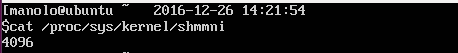
\includegraphics[scale=0.5]{ejercicio1-1.png} 
				\label{figura1} 
				\caption{Archivo history.log}
			\end{figure} 
		\end{itemize} 
	\end{itemize}

	
	\subsection{b) ¿Qué significan las terminaciones .1.gz o .2.gz de los archivos en ese directorio?}
	
	Según las referencias del apartado a), los archivos de log son mantenidos debido a pueden ocupar bastante espacio, sobre todo si fuese un servidor. Crecerían mucho y a la hora de buscar información en un archivo de log sería complicado. Existe un proceso en Linux que rota los archivos de log, renombrando y escribiendo en un nuevo archivo de log. Esto se realiza gracias a una tarea de cron\cite{ejercicio1-9} (ejecuta tareas cada cierto tiempo), que utiliza logrotate\cite{ejercicio1-10} (rota y comprime registros del sistema). De este modo, los archivos son rotados y comprimidos según su antigüedad, evitando que un archivo de log sea muy grande. Así por ejemplo .1.gz tendría información más actualizada que .2.gz.
	\\
	
	Comprobamos el contenido de 2 archivos de log y vemos que aquel que tiene un número con extensión menor es el más actualizado.
	
	\begin{figure}[H] 
		\centering
		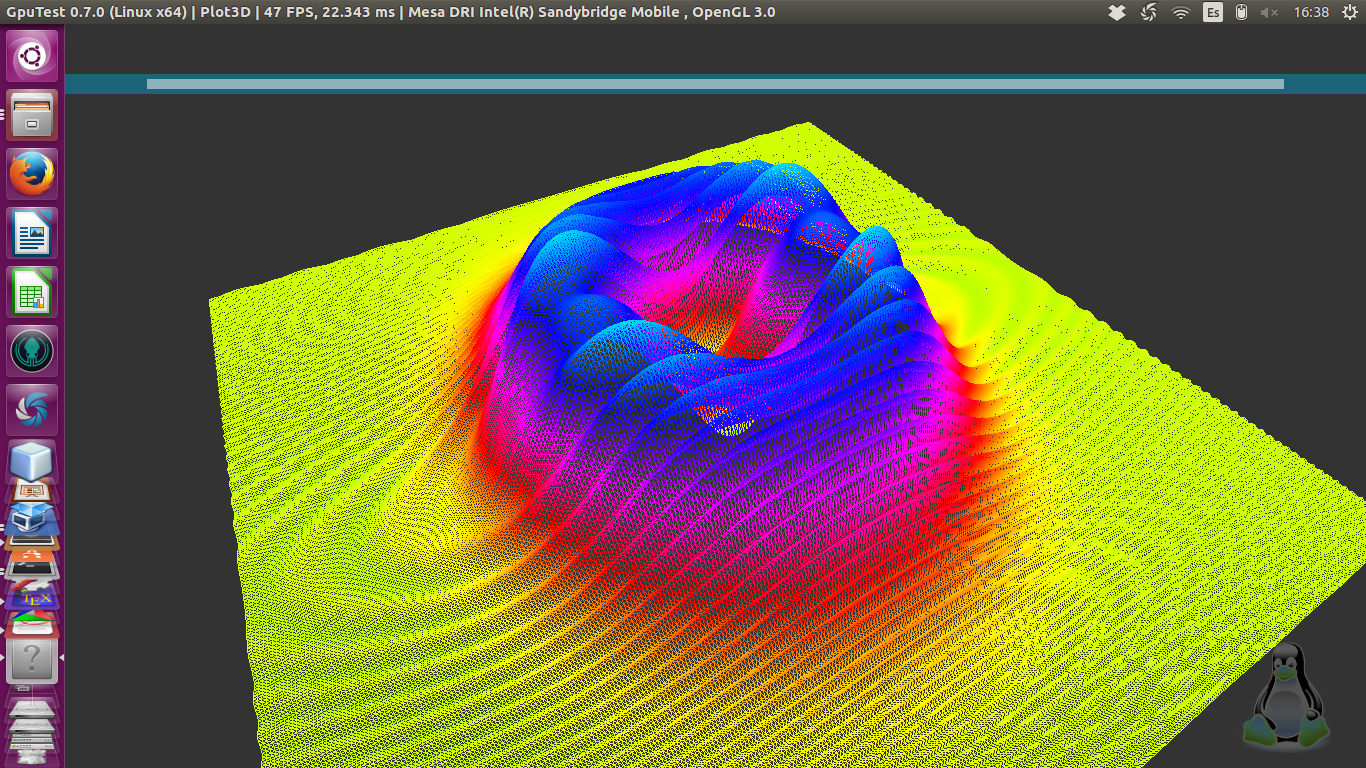
\includegraphics[scale=0.35]{ejercicio1-2.png} 
		\label{figura2} 
		\caption{Comparando antigüedad archivos de log apt}
	\end{figure} 
	
	%----------------------------------------------------------------------------------------
	%	Cuestión 2
	%----------------------------------------------------------------------------------------
	
	\section{¿qué archivo ha de modificar para programar una tarea?Escriba la línea necesaria para ejecutar una vez al día una copia del directorio ~/codigo a ~/seguridad/\$fecha donde \$fecha es la fecha actual(puede usar el comando date).}
	
	
	El archivo a modificar es en /etc/cronab o ejecutando crontab -e\cite{ejercicio2-1}.
	
	Escribimos un script llamado ejercicio2.sh para lo que nos piden:
	\begin{figure}[H] 
		\centering
		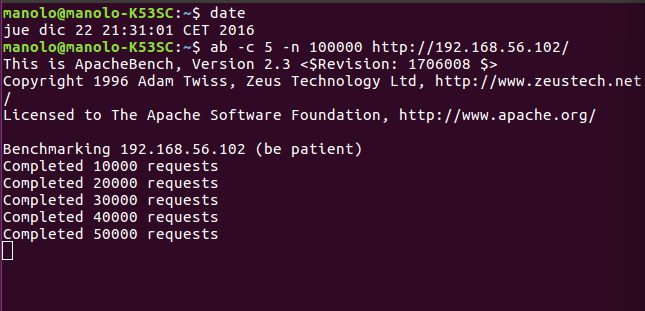
\includegraphics[scale=0.35]{ejercicio2-1.png} 
		\label{figura2} 
		\caption{Script para crontab}
		
	Modificamos crontab para que ejecute el script:
	\end{figure}
	
		\begin{figure}[H] 
			\centering
			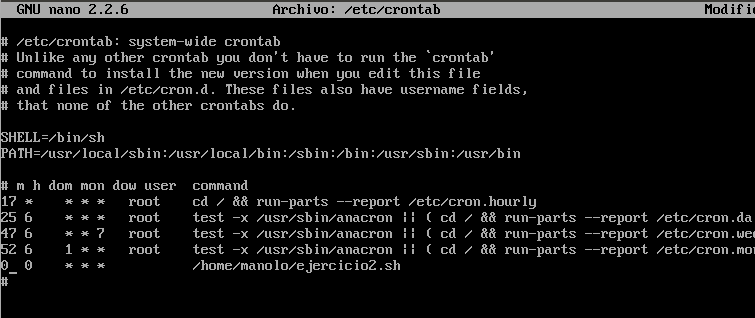
\includegraphics[scale=0.35]{ejercicio2-2.png} 
			\label{figura2} 
			\caption{Modificando crontab}
		\end{figure}
	%----------------------------------------------------------------------------------------
	%	Cuestión 3
	%----------------------------------------------------------------------------------------
	
	\section{Pruebe a ejecutar el comando, conectar un dispositivo USB y vuelva a ejecutar el comando. Copie y pegue la salida del comando.(considere usar dmesg | tail). Comente qué observa en la información mostrada.}
	
	El comando dmesg\cite{ejercicio3-1} muestra información sobre el buffer que está conectado con el kernel. Usando el comando tail vemos los últimos acontecimientos que pasan en el kernel:
	
	\begin{figure}[H] 
		\centering
		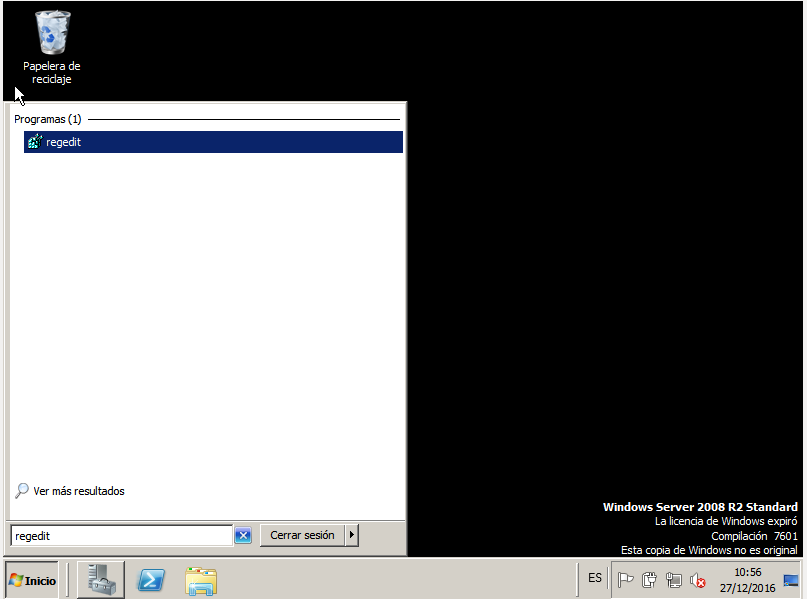
\includegraphics[scale=0.5]{ejercicio3-1.png} 
		\label{figura2} 
		\caption{Desconectando ratón inalámbrico por usb (Logitech)}
	\end{figure}
	
	Vemos como nos dice que el dispositivo USB 2-1-2 está desconectado. Ahora probamos a conectarlo:
	
	\begin{figure}[H] 
		\centering
		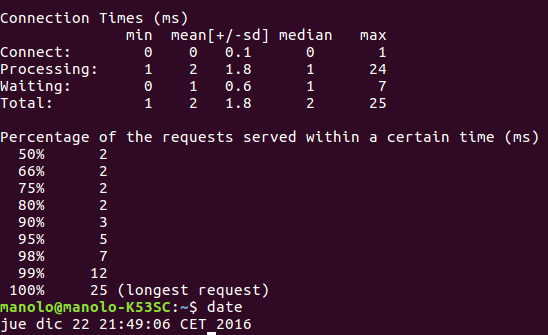
\includegraphics[scale=0.5]{ejercicio3-2.png} 
		\label{figura2} 
		\caption{Conectando ratón inalámbrico por usb (Logitech)}
	\end{figure}
	
	Tras conectarlo, no nos muestra ningún mensaje de que esté desconectado, por lo que todo funciona correctamente.

	%	Cuestión 4
	%-----------------------------------------------
	\section{Ejecute el monitor de “System Performance” y muestre el resultado. Incluya capturas de pantalla comentando la información que aparece.}
	
	Iniciamos Perfmon desde PowerShell. Para ello escribimos en la consola la orden perfmon.
	
	\begin{figure}[H] 
		\centering
		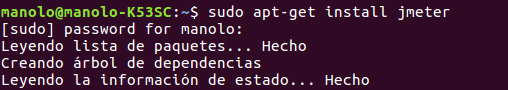
\includegraphics[scale=0.5]{ejercicio4-1.png} 
		\label{figura2} 
		\caption{Abrir Perfmon con PowerShell}
	\end{figure}
	
	Se abrirá el monitor "System Performance" de Windows Server y podemos ver cierta información.
	\begin{figure}[H] 
		\centering
		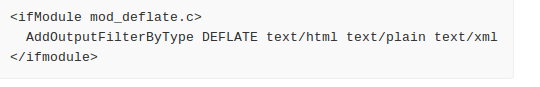
\includegraphics[scale=0.5]{ejercicio4-2.png} 
		\label{figura2} 
		\caption{Monitor System Performance}
	\end{figure}
	
	Tenemos un resumen del sistema donde nos muestra información sobre:
	\begin{itemize}
		\item Disco físico. Muestra por ejemplo el porcentaje de tiempo inactivo. 
			\begin{figure}[H] 
				\centering
				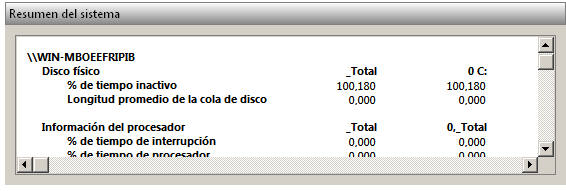
\includegraphics[scale=0.5]{ejercicio4-3.png} 
				\label{figura2} 
				\caption{Perfmon. Resumen de disco físico}
			\end{figure}	
		\item Información del procesador. En este caso la foto muestra porcentajes de tiempos de interrupción y de procesador.
			\begin{figure}[H] 
				\centering
				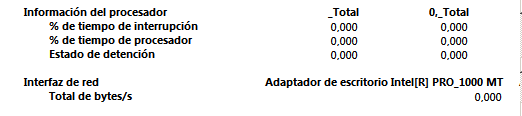
\includegraphics[scale=0.5]{ejercicio4-4.png} 
				\label{figura2} 
				\caption{Perfmon. Resumen de información del procesador}
			\end{figure}
		\item Interfaz de red y memoria. Para la red se muestran los bytes totales usados, pero son 0 porque no estamos haciendo uso de la red. Por otro lado, la memoria por ejemplo nos indica el porcentaje de bytes en uso, que en este caso son 50,662.
			\begin{figure}[H] 
				\centering
				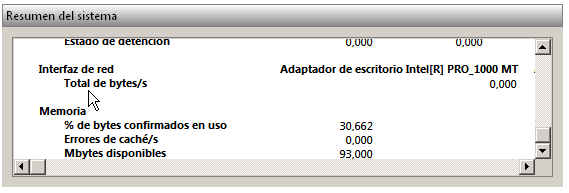
\includegraphics[scale=0.5]{ejercicio4-5.png} 
				\label{figura2} 
				\caption{Perfmon. Resumen de interfaz de red y memoria}
			\end{figure}
	\end{itemize}
	
	
	Perfmon tiene un monitor de rendimiento que nos muestra de forma gráfica la información total del procesador/tiempo de procesador. Vemos como en el eje X nos muestra la hora actual y en el eje Y nos muestra el uso del procesador. Por ejemplo si abrimos el navegador o realizamos alguna acción, el cambio en la gráfica será notable.
	\begin{figure}[H] 
		\centering
		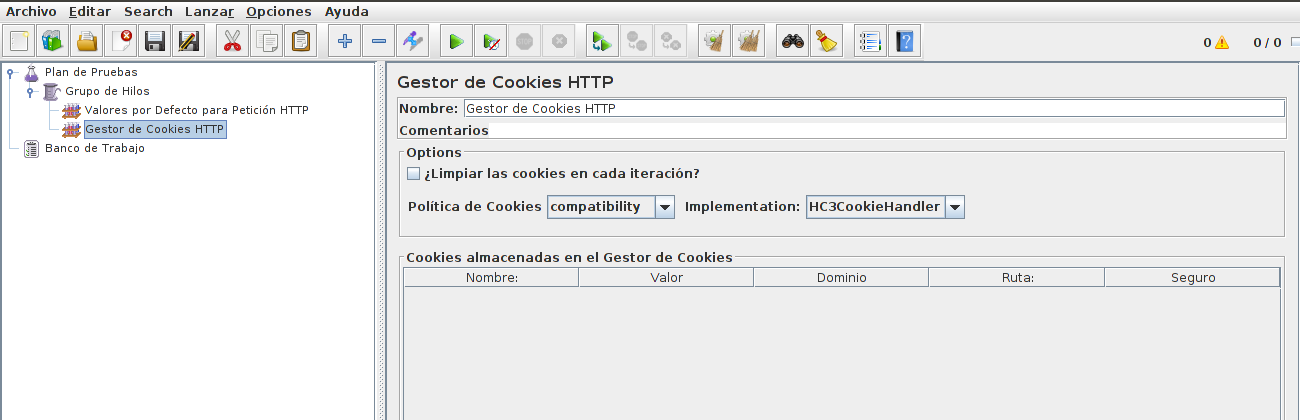
\includegraphics[scale=0.5]{ejercicio4-6.png} 
		\label{figura2} 
		\caption{Perfmon. Monitor de rendimiento}
	\end{figure}
	
	También tenemos recopiladores de datos del sistema, que son:
	\begin{itemize}
		\item Diagnóstico del sistema.
			\begin{figure}[H] 
				\centering
				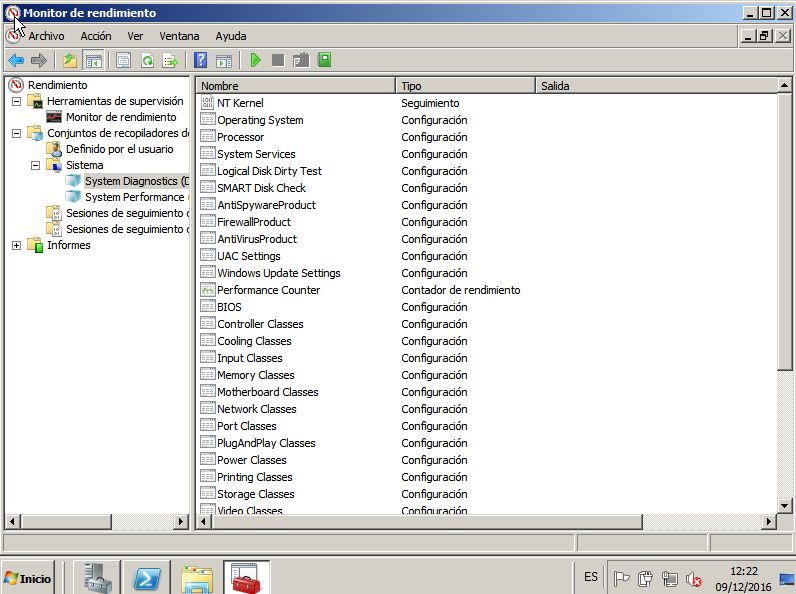
\includegraphics[scale=0.5]{ejercicio4-7.png} 
				\label{figura2} 
				\caption{Perfmon. Recopilador de diagnóstico del sistema}
			\end{figure}
		\item Rendimiento del sistema.
			\begin{figure}[H] 
				\centering
				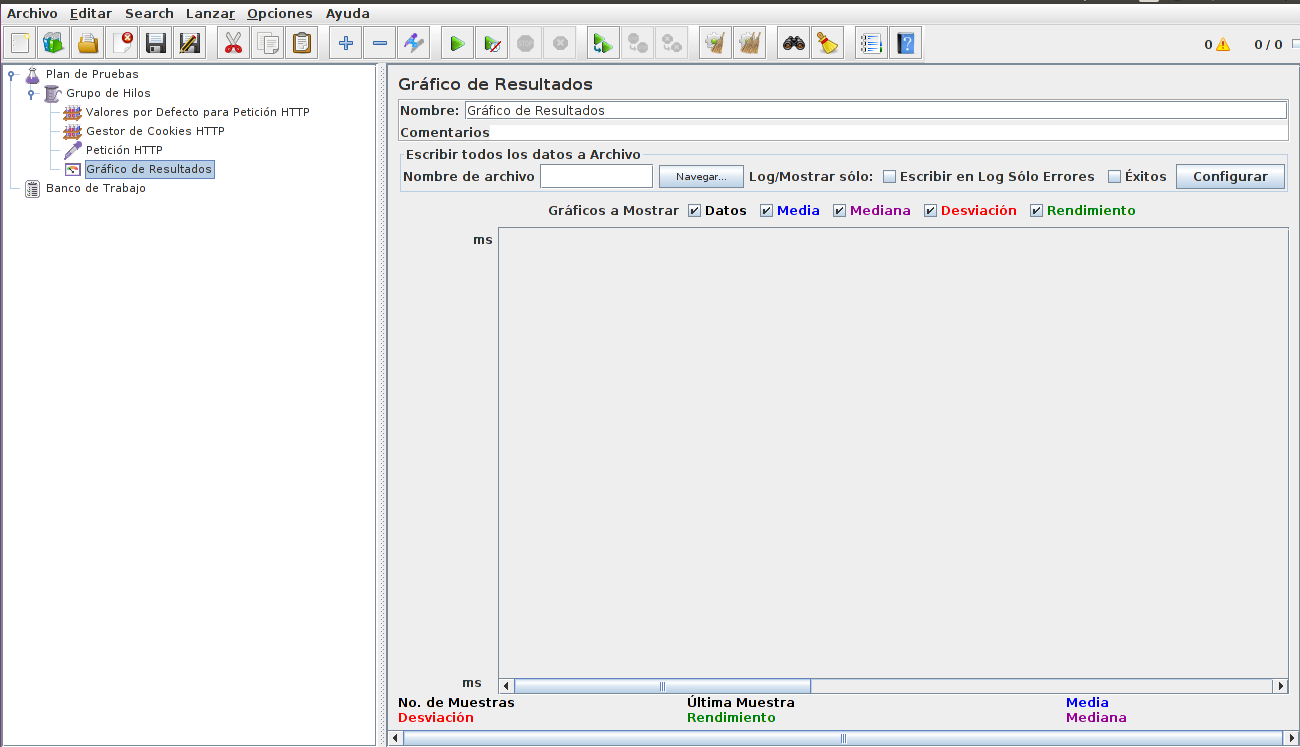
\includegraphics[scale=0.5]{ejercicio4-8.png} 
				\label{figura2} 
				\caption{Perfmon. Recopilador de rendimiento del sistema}
			\end{figure}
	\end{itemize}
	
	%----------------------------------------------------------------------------------------
	%	Cuestión 5
	%----------------------------------------------------------------------------------------
	
	\section{Cree un recopilador de datos definido por el usuario (modo avanzado) que incluya tanto el contador de rendimiento como los datos de seguimiento:Todos los referentes al procesador, al proceso y al servicio web. Intervalo de muestra 15 segundos. Almacene el resultado en el directorio Escritorio /logs. Incluya las capturas de pantalla de cada paso.}
	
	Vamos a ir paso por paso explicando como hacer un recopilador de datos:
	\begin{itemize}
		\item \textbf{Paso 1}: Hacemos click derecho sobre conjuntos de recopiladores del sistema > definidos por el usuario. Nos aparecerá la opción para nuevo > conjunto de recopiladores de datos. Pulsamos y empezamos a configurar el recopilador.
			\begin{figure}[H] 
				\centering
				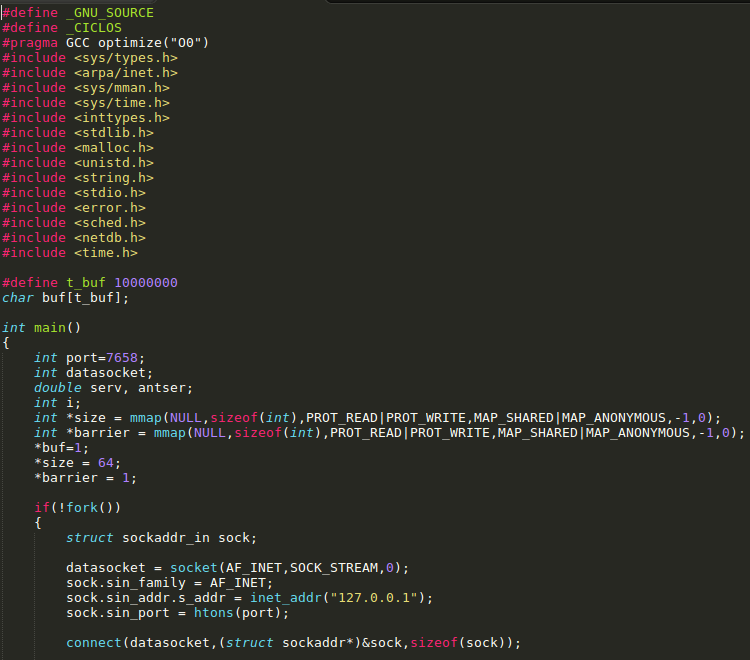
\includegraphics[scale=0.5]{ejercicio5-1.png} 
				\label{figura2} 
				\caption{Paso 1. Crear nuevo recopilador de datos}
			\end{figure}
		\item \textbf{Paso 2}: Elegimos un nombre para el recopilador de datos, por ejemplo "Copilador de datos ISE" y seleccionamos la opción de "Crear manualmente(avanzado)".
			\begin{figure}[H] 
				\centering
				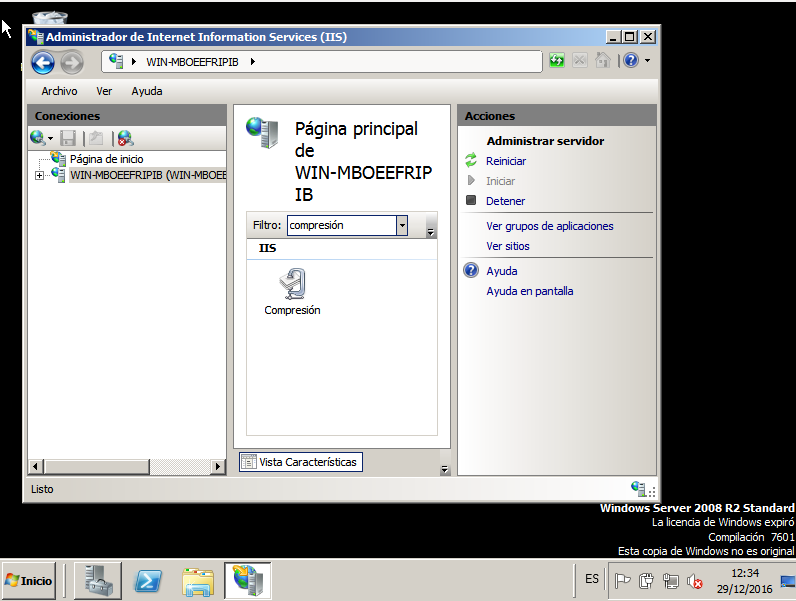
\includegraphics[scale=0.5]{ejercicio5-2.png} 
				\label{figura2} 
				\caption{Paso 2. Establecer nombre y comenzar configuración manual del recopilador de datos}
			\end{figure}
		\item \textbf{Paso 3}: Incluimos los datos que queremos para el recopilador. En este caso, el ejercicio nos pide que elegir "Contador de rendimiento" y "Datos de seguimiento de eventos", por lo que elegimos estos.
			\begin{figure}[H] 
				\centering
				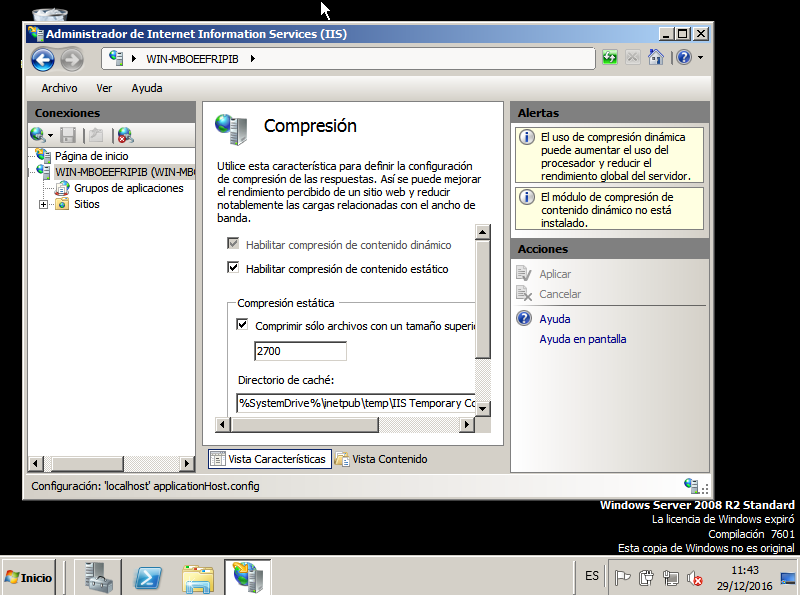
\includegraphics[scale=0.5]{ejercicio5-3.png} 
				\label{figura2} 
				\caption{Paso 3. Incluir registros de datos en el recopilador}
			\end{figure}
		\item \textbf{Paso 4}: Nos aparece una nueva pantalla para incluir contadores de rendimiento al recopilador de datos. Pulsamos en agregar para realizarlo.
			\begin{figure}[H] 
				\centering
				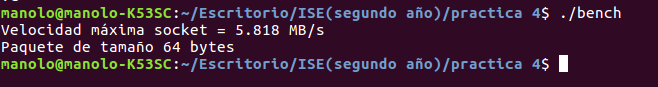
\includegraphics[scale=0.5]{ejercicio5-4.png} 
				\label{figura2} 
				\caption{Paso 4. Registrar contadores de rendimiento}
			\end{figure}
		\item \textbf{Paso 5}: Agregamos los contadores de procesador, proceso y servicio web. Aceptamos para terminar.
			\begin{figure}[H] 
				\centering
				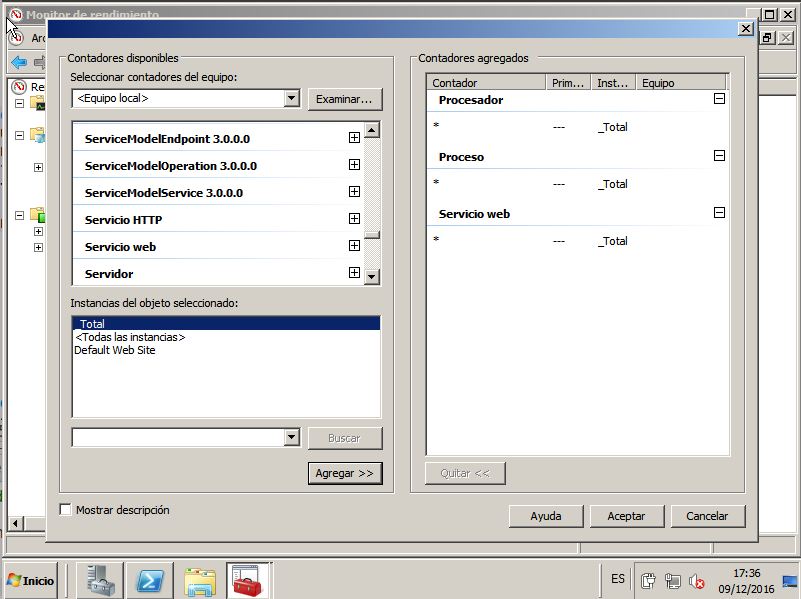
\includegraphics[scale=0.5]{ejercicio5-5.png} 
				\label{figura2} 
				\caption{Paso 5. Agregar contadores de rendimiento}
			\end{figure}
		\item \textbf{Paso 6}: Comprobamos que los contadores que agregamos están presentes. Establecemos el intervalo de muestra a 15s como pide en el guión de prácticas y continuamos y pulsamos siguiente.
			\begin{figure}[H] 
				\centering
				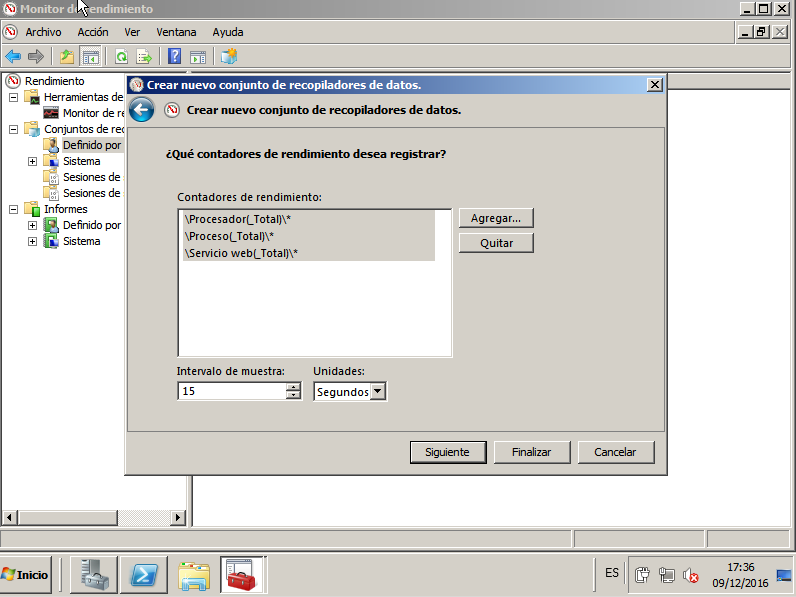
\includegraphics[scale=0.5]{ejercicio5-6.png} 
				\label{figura2} 
				\caption{Paso 6. Finalizar agregación de contadores de rendimiento}
			\end{figure}
		\item \textbf{Paso 7}: Nos aparece una pantalla para habilitar proveedores de seguimiento. No tenemos que agregar ninguno, por lo que le damos a siguiente.
			\begin{figure}[H] 
				\centering
				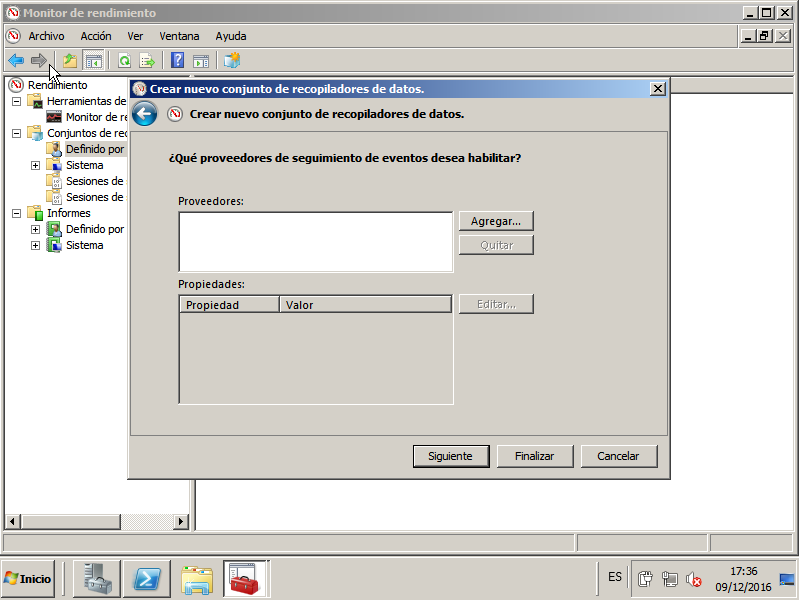
\includegraphics[scale=0.5]{ejercicio5-7.png} 
				\label{figura2} 
				\caption{Paso 7. Habilitar proveedores de seguimiento}
			\end{figure}
		\item \textbf{Paso 8}: Ahora nos pide una ruta donde guardar los datos del recopilador. Para ello vamos a crear una carpeta en Escritorio que se llame "logs" tal y como nos pide en el guión. Tras crearla le indicamos que sea esa carpeta el directorio raíz.
			\begin{figure}[H] 
				\centering
				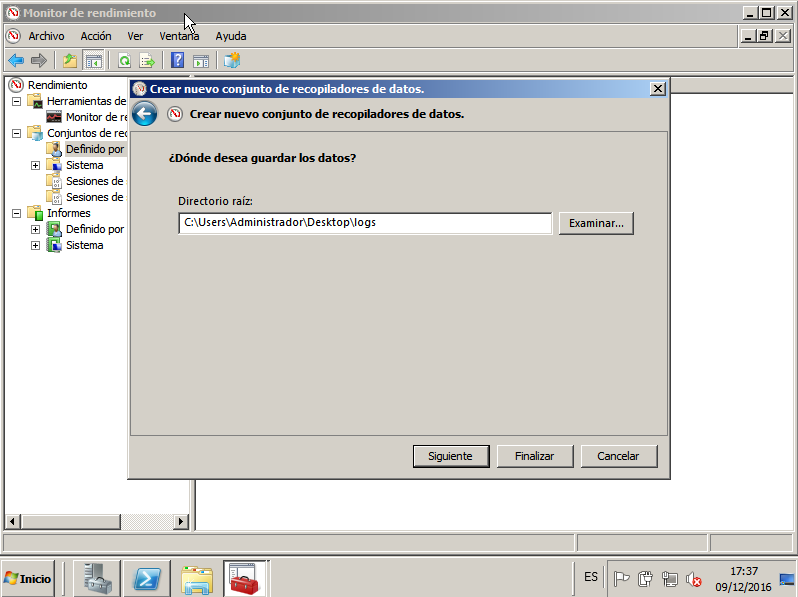
\includegraphics[scale=0.5]{ejercicio5-8.png} 
				\label{figura2} 
				\caption{Paso 8. Ruta para guardar los datos de recopilador}
			\end{figure}
		\item \textbf{Paso 9}: Finalizar la creación del conjunto de recopiladores de datos. Pulsamos finalizar y se creará.
			\begin{figure}[H] 
				\centering
				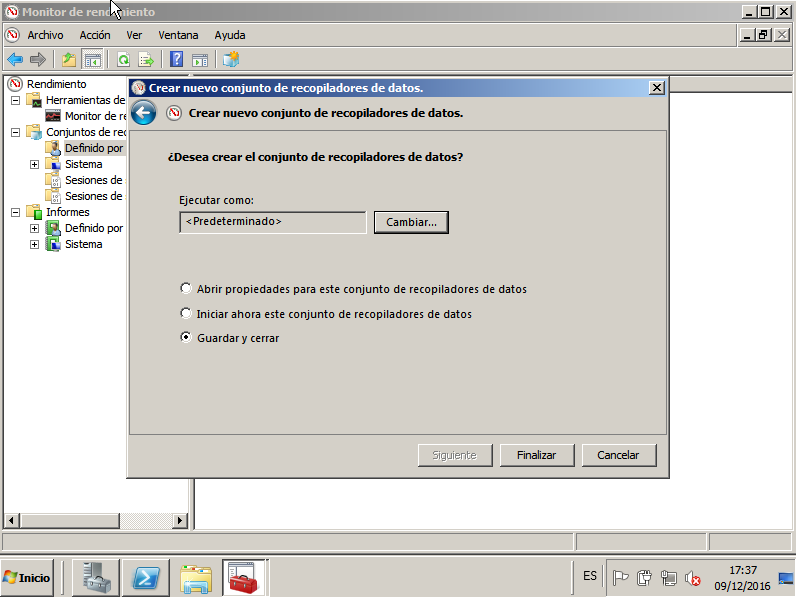
\includegraphics[scale=0.5]{ejercicio5-9.png} 
				\label{figura2} 
				\caption{Paso 9. Finalizar creación del recopilador de datos}
			\end{figure}
	\end{itemize}
	
	
	Comprobamos que el recopilador ha sido creado. Se encontrará dentro de Conjuntos de recopiladores de datos > Definido por el usuario.
	\begin{figure}[H] 
		\centering
		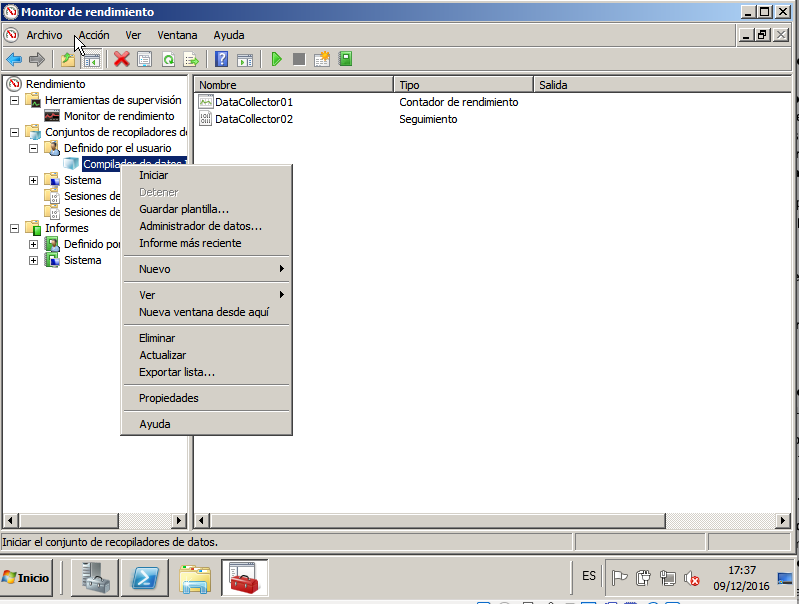
\includegraphics[scale=0.5]{ejercicio5-10.png} 
		\label{figura2} 
		\caption{Comprobar la creación del recopilador de datos}
	\end{figure}
	
	Hacemos click derecho sobre él y nos permitirá la opción de iniciar. De este modo empezar a recopilar datos. Esperaremos unos minutos para que lo haga y lo pararemos dandole a "Detener".\\
	
	Vamos a ver que ha generado. Para ello nos vamos a Informes > Definido por el usuario > Copilador de datos ISE. Nos aparecerá un informe que al pulsa sobre él nos mostrará la siguiente gráfica:
	\begin{figure}[H] 
		\centering
		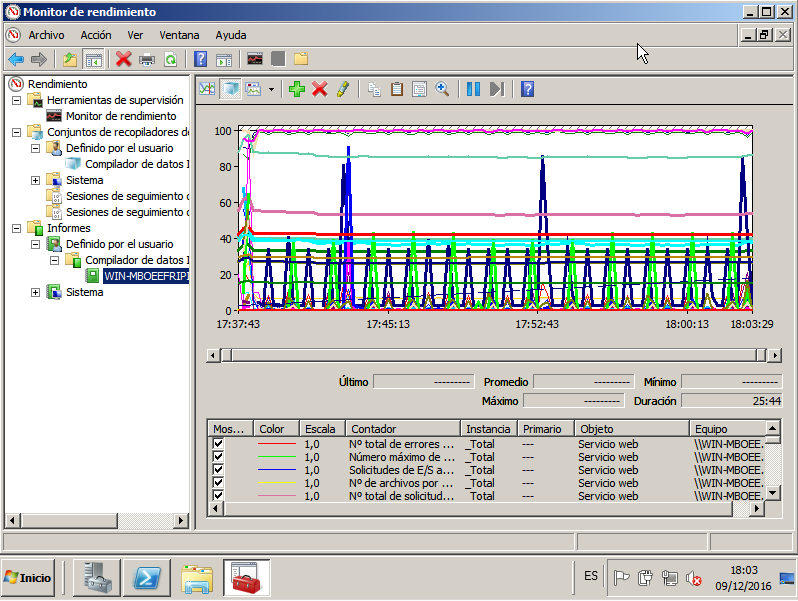
\includegraphics[scale=0.5]{ejercicio5-11.png} 
		\label{figura2} 
		\caption{Gráfico generado por el recopilador de datos}
	\end{figure}
	
	Por ejemplo, vamos a comprobar los datos recopilados del servicio web. Vemos como tenemos abajo del gráfico una lista con todo lo que nos muestra, de modo que dejamos únicamente los objetos de servicio web. Vemos como no ha habido actividad en nada del servicio web.
	\begin{figure}[H] 
		\centering
		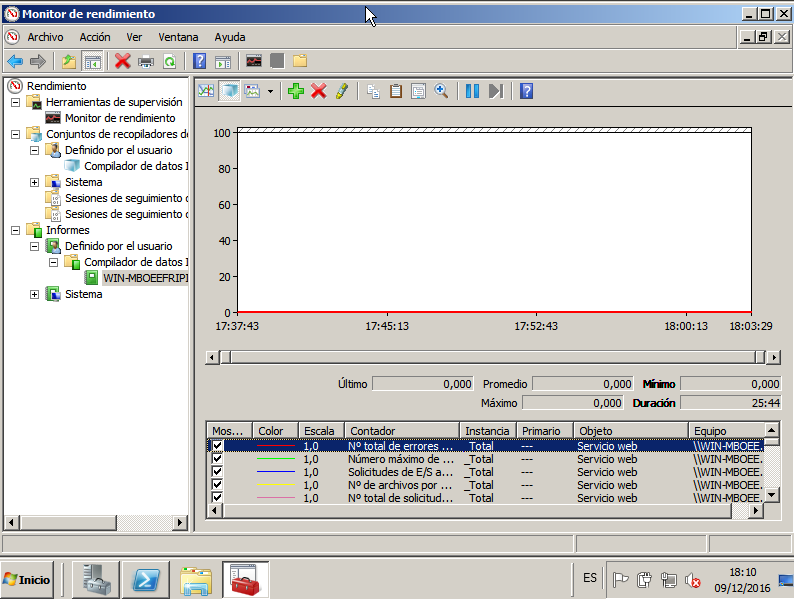
\includegraphics[scale=0.5]{ejercicio5-12.png} 
		\label{figura2} 			
		\caption{Gráfico generado solo para servicio web}
	\end{figure}
	
	Vamos a ver en los procesos las operaciones de E/S para datos, escritura y lectura. En color azul datos, en color carne lectura y en violeta escritura. Vemos como las E/S de datos han sido mayores que las de lectura (que son las segundas) y de escritura (las últimas). A las 17:43 la E/S de datos tiene un máximo de 90,920 ya que abrí el navegador "Internet Explorer" en ese momento. Ese ha sido su único periodo de más actividad, ya que luego presenta picos de procesador mas inferiores entre 5 y 6 regularmente.\\
	Por otra parte, la E/S de lectura tiene picos muy pequeños durante todo el periodo de recopilación de datos, teniendo valores de procesador entorno a 3 y 4.\\
	Finalmente la E/S de escritura es la más inferior, ya que en el periodo de medición la única escritura realizada era en los archivos del propio recopilador. Igual para la E/S de lectura, y para la de datos, por eso sus gráficas son similares excepto en un momento puntual (máximo de E/S de datos).
	
	\begin{figure}[H] 
		\centering
		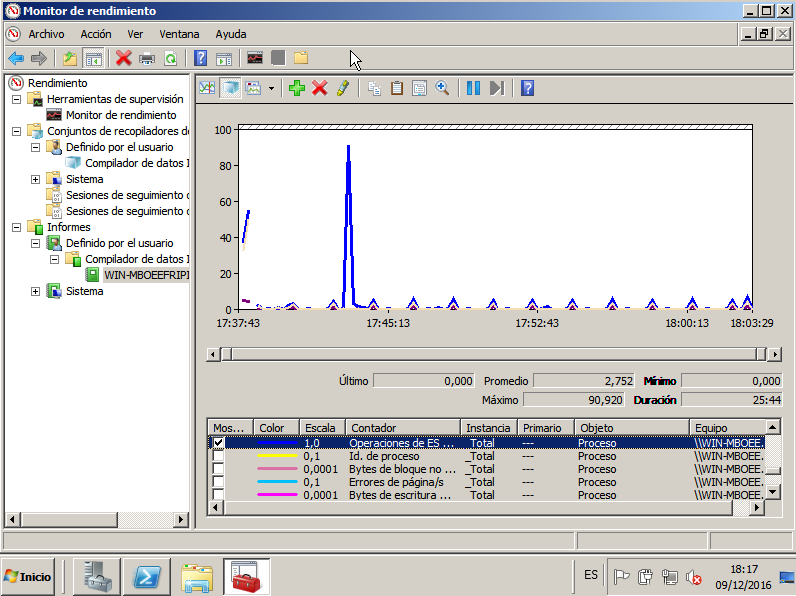
\includegraphics[scale=0.5]{ejercicio5-13.png} 
		\label{figura2} 			
		\caption{Gráfico generado solo para E/S de procesos}
	\end{figure}
	%----------------------------------------------------------------------------------------
	%	Cuestión 6
	%----------------------------------------------------------------------------------------
	
	\section{Visite la web del proyecto y acceda a la demo que proporcionan (http://demo.munin-monitoring.org/) donde se muestra cómo monitorizan un servidor. Monitorice varios parámetros y haga capturas de pantalla de lo que está mostrando comentando qué observa.}
	
	
	Munin\cite{ejercicio6-1} permite monitorizar parámetros relacionados con  disco, procesos o el sistema, recopilar sus datos durante diferentes periodos (días, semanas, meses o años) y realizar un seguimiento gráfico de dichos.\\
	
	Por ejemplo vamos a ver un gráfico sobre el estado de los procesos de un servidor en un día.\\
	Vemos como en el eje X se representan las horas del día y en el eje Y el número de procesos. Esta gráfica nos muestra que casi la totalidad de procesos del servidor están durmiendo (actualmente 71) teniendo una media de 72.22 procesos durmiendo durante un día concreto. Podemos ver que tiene solo 1 proceso ejecutándose actualmente y que la media de procesos ejecutándose es solo 1. Los demás estados de los procesos no han ocurrido, por lo que no se ven gráficamente.\\
	
	La conclusión de esta gráfica es que la CPU del servidor no está consumiendo muchos recursos ya que solo tiene un proceso activo.
	\begin{figure}[H] 
		\centering
		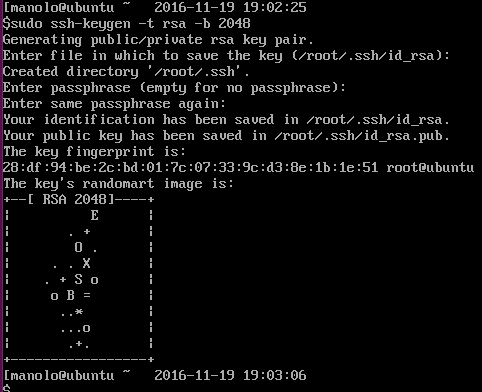
\includegraphics[scale=0.5]{ejercicio6-1.png} 
		\label{figura2} 			
		\caption{Gráfico de estado de los procesos durante un día}
	\end{figure}


	Vamos a ver ahora una gráfica del sistema referente al uso de disco en un periodo de un mes. Vemos que el disco ha sido utilizado solo por el root con una media de uso del 31.57 \%.
	\begin{figure}[H] 
		\centering
		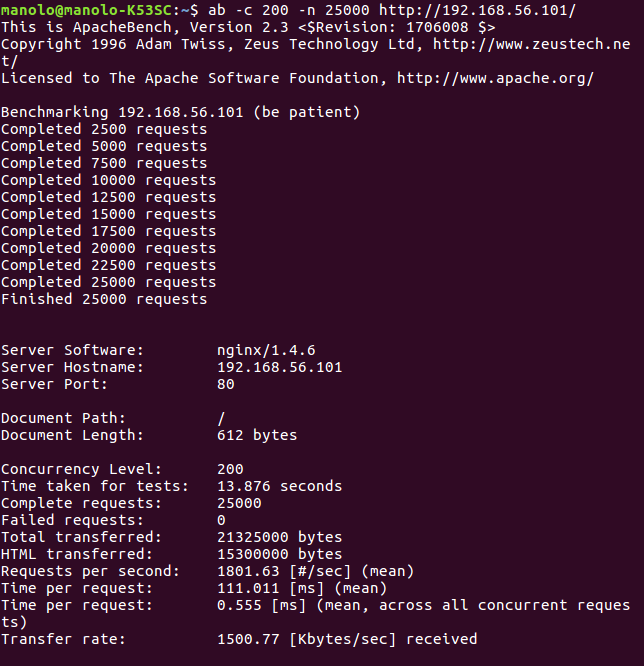
\includegraphics[scale=0.5]{ejercicio6-2.png} 
		\label{figura2} 			
		\caption{Uso de disco del servidor durante un mes}
	\end{figure}


	Observemos otra gráfica sobre el uso de memoria durante un mes. Vemos como quienes más usan la memoria son commited (memoria asignada a programas), inactive (memoria no usada), active (memoria usada recientemente) y apps (memoria usada por aplicaciones en espacio de usuario). Quienes menos la usan son shemem (memoria compartida), page tables (memoria para mapear entre direcciones físicas y lógicas) y unused (memoria perdida, que no es usada para nada).\\
	
	Como conclusión, el servidor tiene mucha memoria dedica a los programas y aplicaciones de usuario. Tiene una cantidad importante de memoria no usada, por lo que la memoria no está completamente llena y otra parte de memoria que es usada con frecuencia, lo que hace destacar que el servidor tiene actividad.
	\begin{figure}[H] 
		\centering
		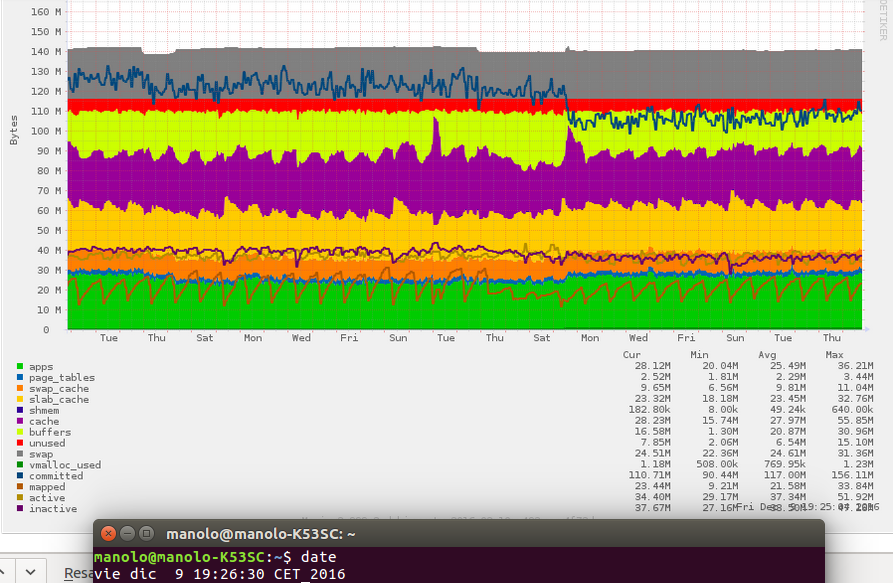
\includegraphics[scale=0.5]{ejercicio6-3.png} 
		\label{figura2} 			
		\caption{Uso de memoria del servidor durante un mes}
	\end{figure}
	\begin{figure}[H] 
		\centering
		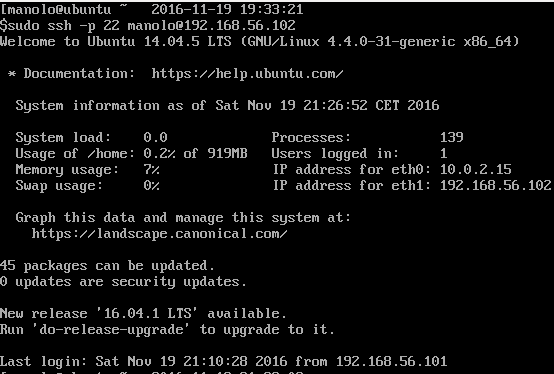
\includegraphics[scale=0.5]{ejercicio6-4.png} 
		\label{figura2} 			
		\caption{Información de la tabla de memoria}
	\end{figure}
	%----------------------------------------------------------------------------------------
	%	Cuestión 7
	%----------------------------------------------------------------------------------------
	\section{Escriba un breve resumen sobre alguno de los artículos donde se muestra el uso de strace o busque otro y coméntelo.}
	
	Strace nos sirve para hacer un seguimiento de las llamadas al sistema realizadas por algún procedimiento (seguir un flujo de llamadas), permitiendo así comprobar si hay errores durante dichas llamadas, permitiendo de este modo resolver problemas relacionados con dicho 
	procedimiento.\\
	
	Este comando podría usarse para un comando o un archivo ejecutable. Para ver como realiza el seguimiento voy a hacer un ejemplo con ls\cite{ejercicio7-1}:
	\begin{center}
		\$ \textbf{strace ls}
	\end{center}
	\begin{figure}[H] 
		\centering
		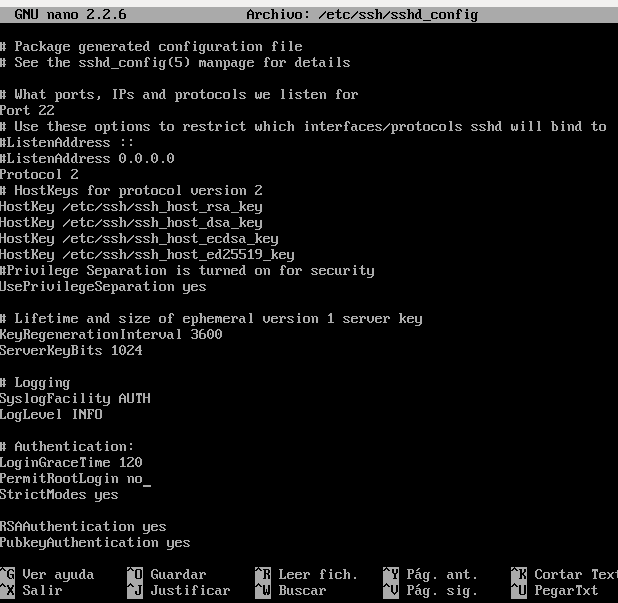
\includegraphics[scale=0.35]{ejercicio7-1.png} 
		\label{figura2} 			
		\caption{Uso de strace para ls}
	\end{figure}
	
	Vemos como ls realiza llamadas al sistema como open(), close(), fstat() para tener información del estado de los archivos, mmap() para asignar o quitar archivos o dispositivos a la memoria con el fin de obtener como resultado lo que se espera de él, obtener la lista de archivos que hay en un directorio.
	%----------------------------------------------------------------------------------------
	%	Cuestión 8
	%----------------------------------------------------------------------------------------
	\section{Escriba un script en Python o PHP y analice su comportamiento usando el profiler presentado.}
	
	Voy a realizar un script en Python\cite{ejercicio8-1} que realiza un bucle con 90000 iteraciones. El contenido del script es el siguiente:
	\begin{figure}[H] 
		\centering
		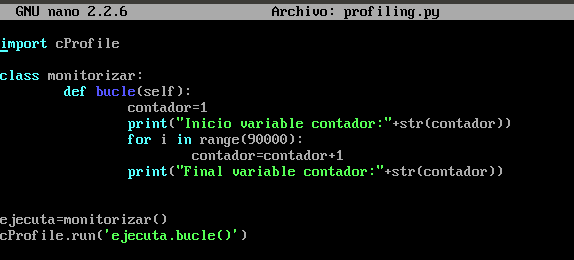
\includegraphics[scale=0.35]{ejercicio8-1.png} 
		\label{figura2} 			
		\caption{Script en Python para profiler}
	\end{figure}
	
	Ejecutamos el profiler para ver que información nos muestra:
	\begin{figure}[H] 
		\centering
		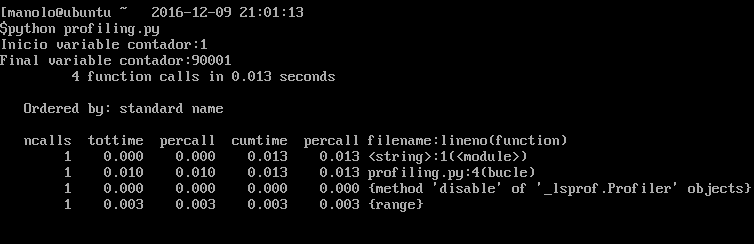
\includegraphics[scale=0.35]{ejercicio8-2.png} 
		\label{figura2} 			
		\caption{Ejecutando profiler en Python}
	\end{figure}
	
	Vemos como ejecuta el script y muestra la información de salida que tenía y además el profiler nos da datos sobre las llamadas que se realizan o por ejemplo el tiempo que tardó por llamada o el tiempo total.
	%----------------------------------------------------------------------------------------
	%	Cuestión 9
	%----------------------------------------------------------------------------------------
	\section{Acceda a la consola mysql (o a través de phpMyAdmin) y muestre el resultado de mostrar el ”profile” de una consulta (la creación de la BD y la consulta la puede hacer libremente).}
	
	Vamos a crear unas tablas y a realizar un par de operaciones en mysql para despues mostrar el "profile"\cite{ejercicio9-1}.

	\begin{itemize}
		\item sudo mysql -p . Para acceder a mysql.
			\begin{figure}[H] 
				\centering
				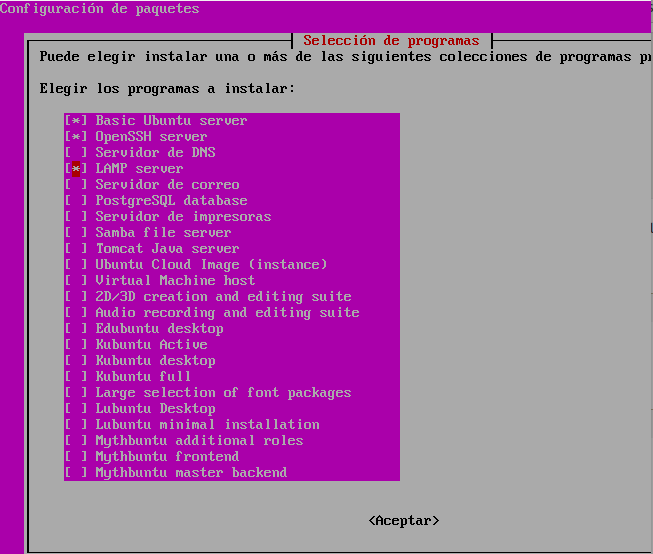
\includegraphics[scale=0.35]{ejercicio9-1.png} 
				\label{figura2} 			
				\caption{Iniciar mysql}
			\end{figure}
		\item mysql> SET profiling = 1; Para poder mostrar profiles.
		\item mysql> CREATE DATABASE ise;
			\begin{figure}[H] 
				\centering
				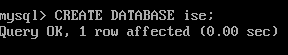
\includegraphics[scale=0.35]{ejercicio9-2.png} 
				\label{figura2} 			
				\caption{Crear base de datos en mysql}
			\end{figure}
		\item mysql> use ise;
			\begin{figure}[H] 
				\centering
				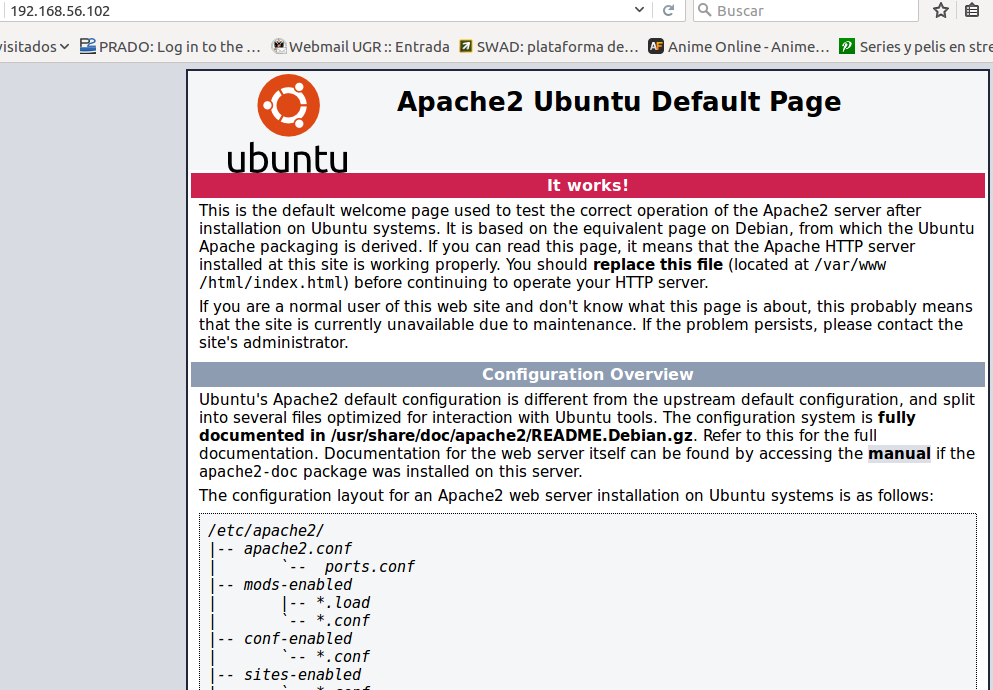
\includegraphics[scale=0.35]{ejercicio9-3.png} 
				\label{figura2} 			
				\caption{Usar una base de datos existente en mysql}
			\end{figure}
		\item mysql> show tables; nos dice que no tenemos
			\begin{figure}[H] 
				\centering
				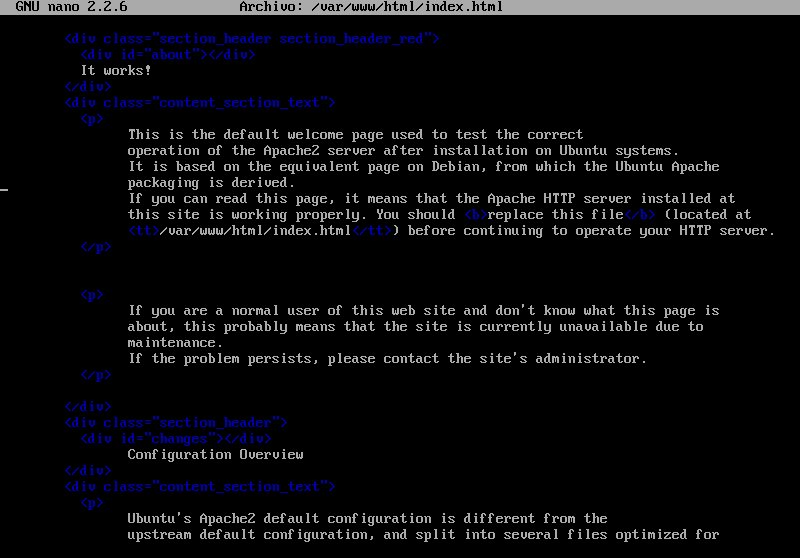
\includegraphics[scale=0.35]{ejercicio9-4.png} 
				\label{figura2} 			
				\caption{Ver tablas de una base de datos en mysql}
			\end{figure}
		\item mysql> create table mascota(nombre VARCHAR(20), propietario VARCHAR(20), especie VARCHAR(20));
			\begin{figure}[H] 
				\centering
				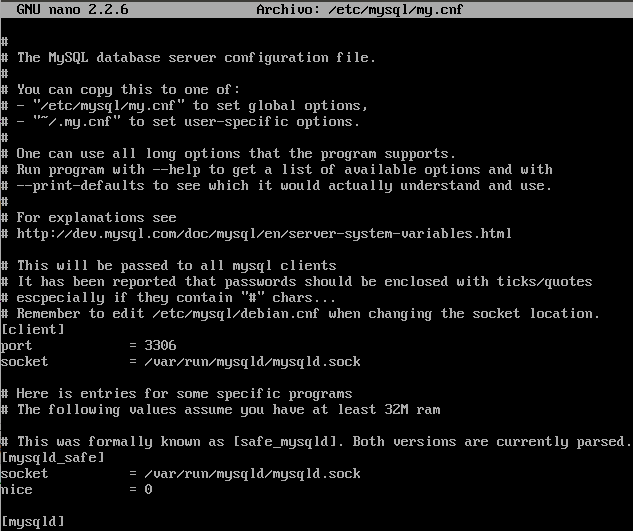
\includegraphics[scale=0.35]{ejercicio9-5.png} 
				\label{figura2} 			
				\caption{Crear tabla en una base de datos en mysql}
			\end{figure}
		\item mysql> insert into mascota  values('lucera','manolo','perro');
			\begin{figure}[H] 
				\centering
				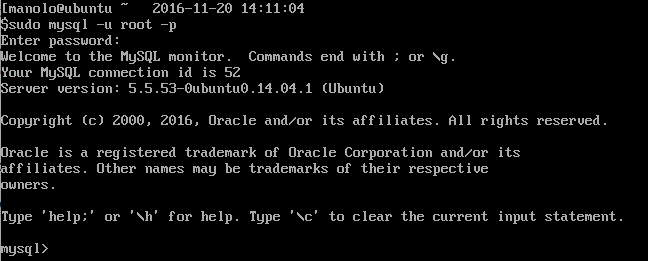
\includegraphics[scale=0.35]{ejercicio9-6.png} 
				\label{figura2} 			
				\caption{Insertar una fila en una tabla en mysql}
			\end{figure}
		\item mysql> insert into mascota values('luna','pepe','gato');
			\begin{figure}[H] 
				\centering
				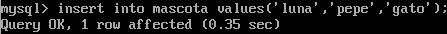
\includegraphics[scale=0.35]{ejercicio9-7.png} 
				\label{figura2} 			
				\caption{Insertar otra fila en una tabla en mysql}
			\end{figure}
		\item mysql> select * from mascota;
			\begin{figure}[H] 
				\centering
				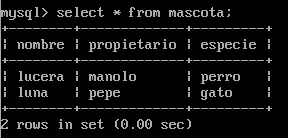
\includegraphics[scale=0.35]{ejercicio9-8.png} 
				\label{figura2} 			
				\caption{Ver tabla mascota en mysql}
			\end{figure}
		\item mysql> show profiles;  (con esto vemos el tiempo de cada operación)
			\begin{figure}[H] 
				\centering
				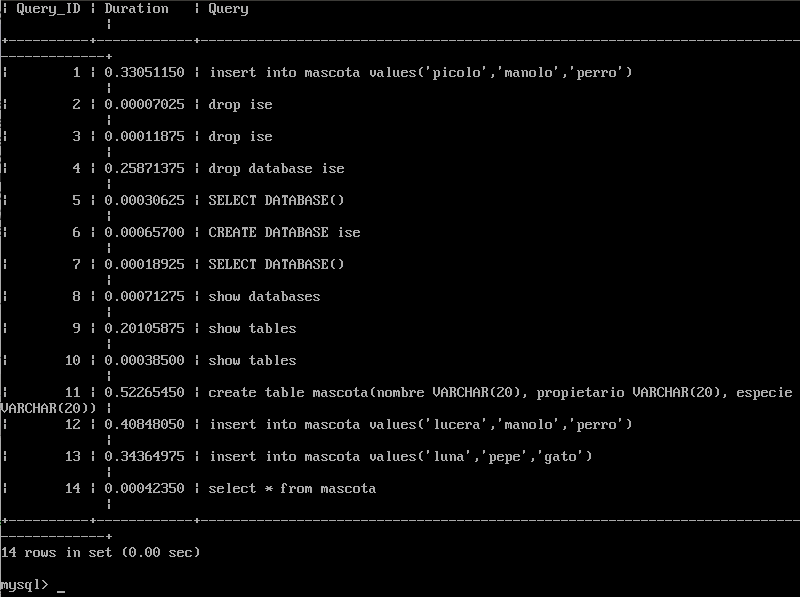
\includegraphics[scale=0.35]{ejercicio9-9.png} 
				\label{figura2} 			
				\caption{Ver profiles en mysql}
			\end{figure}
	\end{itemize}
	
	Vemos como el profile nos muestra el tiempo que ha tardado en realizarse cada operación que hemos realizado en mysql. Vemos que las operaciones más costosas han sido las de creación de la tabla y la de inserción de valores en ella, ya que estamos realizando operaciones de escritura. Vemos como las operaciones de solo lectura como mostrar lo que hay en las tablas son más rápidas.
	%----------------------------------------------------------------------------------------
	%	Cuestión opcional 1
	%----------------------------------------------------------------------------------------
	\section{Opcional 1: Indique qué comandos ha utilizado para realizarlo así como capturas de pantalla del proceso de reconstrucción del RAID.}
	

	%----------------------------------------------------------------------------------------
	%	Cuestión opcional 2
	%----------------------------------------------------------------------------------------
	\section{Opcional 2: Instale Nagios en su sistema (el que prefiera) documentando el proceso y muestre el resultado de la monitorización de su sistema comentando qué aparece.}
	

	%----------------------------------------------------------------------------------------
	%	Cuestión opcional 3
	%----------------------------------------------------------------------------------------
	\section{Opcional 3: Pruebe a instalar este monitor en alguno de sus tres sistemas. Realice capturas de pantalla del proceso de instalación y comente capturas de pantalla del programa en ejecución.}
	
	
	
	%----------------------------------------------------------------------------------------
	%	Cuestión opcional 4
	%----------------------------------------------------------------------------------------
	\section{Opcional 4: Pruebe a instalar este monitor en alguno de sus tres sistemas. Realice capturas de pantalla del proceso de instalación y comente capturas de pantalla del programa en ejecución.}
	
	Vamos a instalar Cacti\cite{opcional4-1} paso por paso:
	
	\begin{itemize}
		\item Instalamos Cacti: sudo apt-get install cacti . Dentro del proceso de instalación nos instalará:
		\begin{itemize}
			\item Nos dará a elegir entre varios servidores, elegiremos Apache2.
			\item Instalará php.
			\item Instalará MySQL.
			\item Otros servicios necesarios para Cacti, como rddtool y snmp.
			\item Configuración de Cacti.
			\begin{itemize}
				\item Configurar la base de datos para Cacti.
				\begin{figure}[H] 
					\centering
					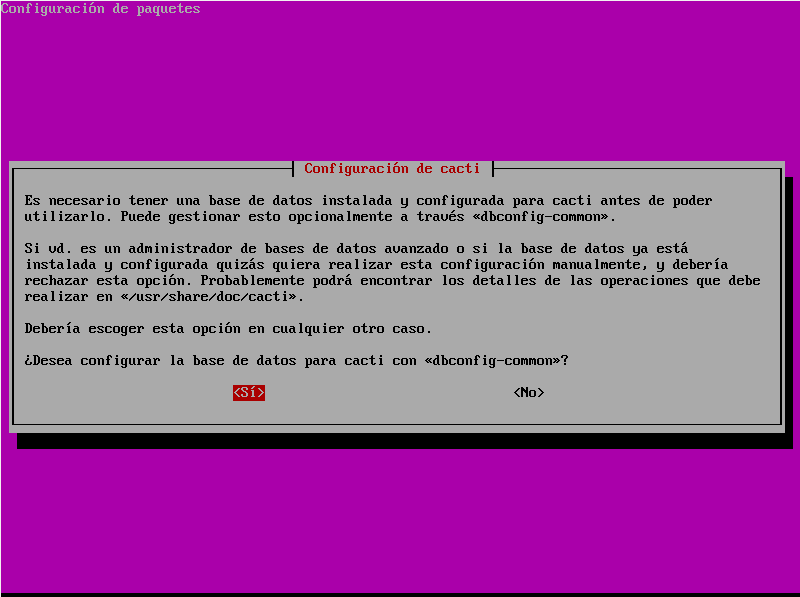
\includegraphics[scale=0.5]{opcional4-1.png} 
					\label{figura2} 			
					\caption{Configurar la base de datos para cacti}
				\end{figure}
				\item Crear contraseña para usuario de administración de la base de datos.
				\begin{figure}[H] 
					\centering
					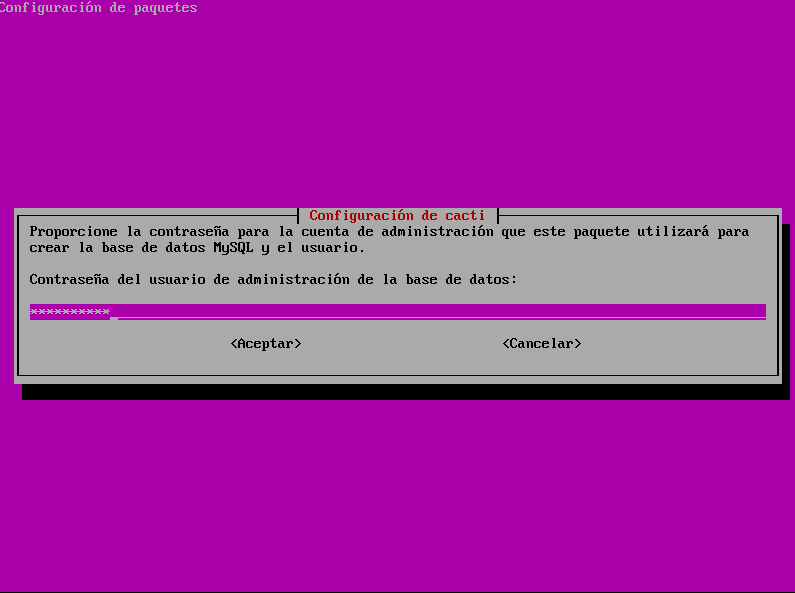
\includegraphics[scale=0.5]{opcional4-2.png} 
					\label{figura2} 			
					\caption{Crear contraseña de administración para BD}
				\end{figure}
				\item Crear contraseña de MySQL para Cacti.
				\begin{figure}[H] 
					\centering
					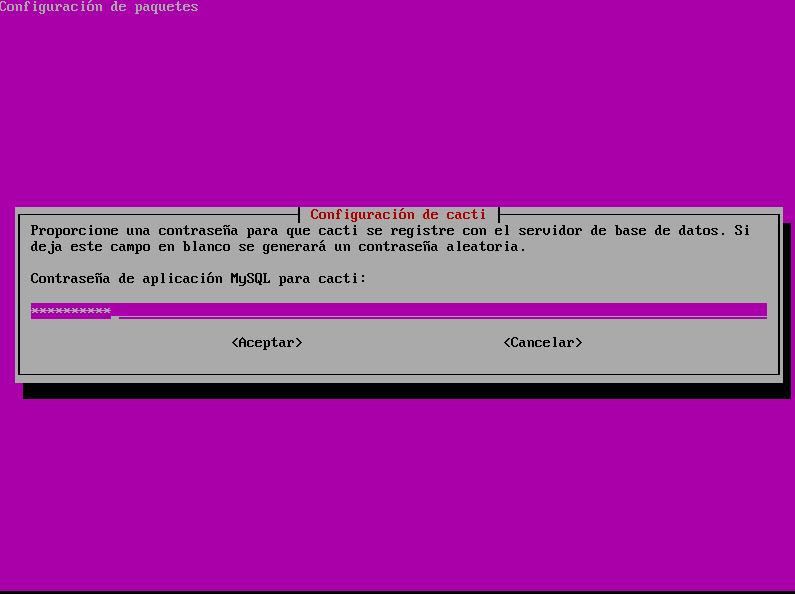
\includegraphics[scale=0.5]{opcional4-3.png} 
					\label{figura2} 			
					\caption{contraseña de MySQL para Cacti}
				\end{figure}
				\item Confirmación de contraseña de MySQL.
				\begin{figure}[H] 
					\centering
					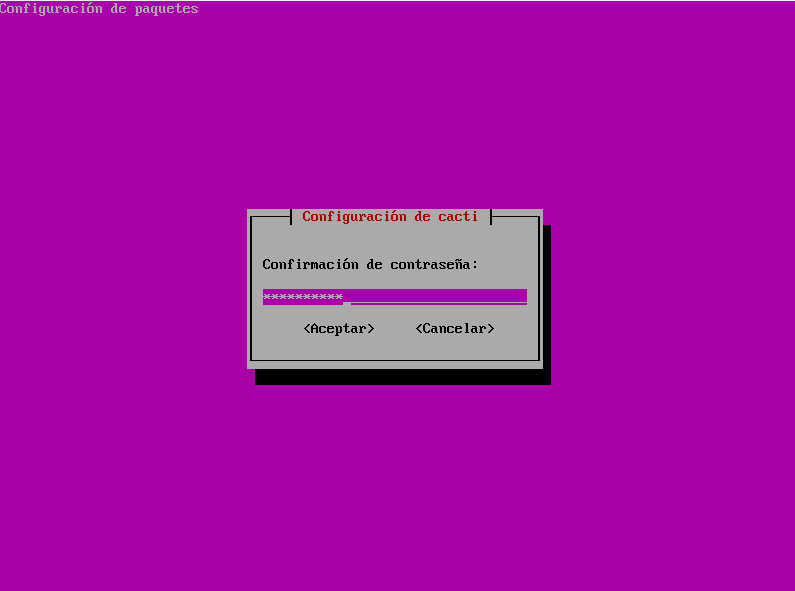
\includegraphics[scale=0.5]{opcional4-4.png} 
					\label{figura2} 			
					\caption{Confirmación de contraseña de MySQL}
				\end{figure}	 
			\end{itemize}
		\end{itemize}
		\item Comprobamos que Cacti ha sido instalado. Para ello, desde la máquina anfitriona nos conectamos a la ip de nuestro servidor escribiendo en el navegador: 192.168.56.102/cacti. Nos pedirá usuario y contraseña (será "admin", "admin" por defecto). Nos pedirá actualizar la contraseña solo con iniciar sesión.\\
		Después de cambiar la contraseña, nos aparecerá una guía de instalación. Aceptamos para pasar a otro paso de instalación 'next' y acabamos 'Finish' para finalizarla:
		\begin{figure}[H] 
			\centering
			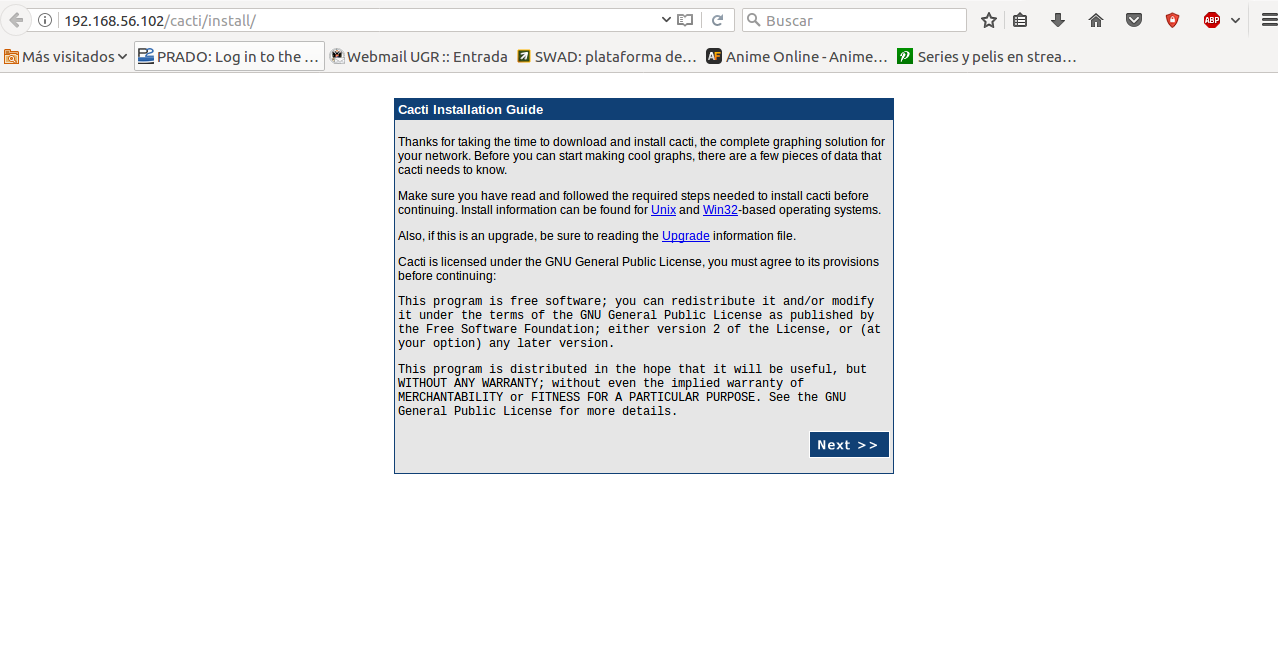
\includegraphics[scale=0.35]{opcional4-5.png} 
			\label{figura2} 			
			\caption{Paso 1 guía instalación Cacti}
		\end{figure}
		\begin{figure}[H] 
			\centering
			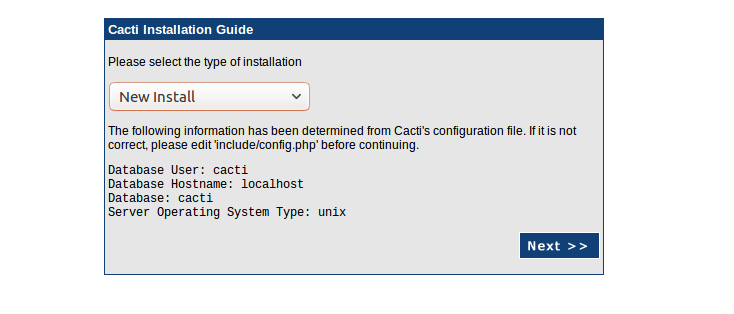
\includegraphics[scale=0.5]{opcional4-6.png} 
			\label{figura2} 			
			\caption{Paso 2 guía instalación Cacti}
		\end{figure}
		\begin{figure}[H] 
			\centering
			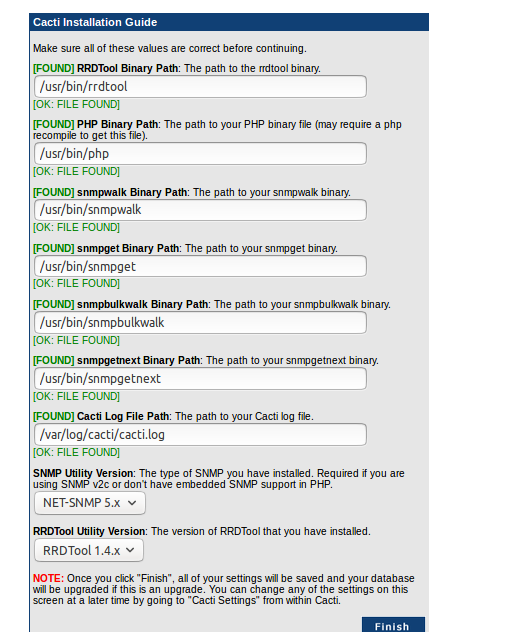
\includegraphics[scale=0.5]{opcional4-7.png} 
			\label{figura2} 			
			\caption{Paso 3 guía instalación Cacti}
		\end{figure}
		\item Vemos la interfaz de Cacti, donde nos muestra las diferentes opciones a realizar. Se pueden crear nuevos gráficos (de varios parámetros del sistema)
		\begin{figure}[H] 
			\centering
			\includegraphics[scale=0.35]{opcional4-8.png} 
			\label{figura2} 			
			\caption{Interfaz de Cacti}
		\end{figure}
		\item Pulsamos sobre las gráficas, mostrándose varias como vemos aquí:
		\begin{itemize}
			\item Carga media del localhost. No hemos generado mucha carga, ya que no hemos realizado ninguna acción que lo requiera.
			\begin{figure}[H] 
				\centering
				\includegraphics[scale=0.5]{opcional4-9.png} 
				\label{figura2} 			
				\caption{Gráfica de carga media de Cacti}
			\end{figure}
			\item Procesos del localhost. La cantidad de procesos ejecutándose en nuestro Ubuntu Server.
			\begin{figure}[H] 
				\centering
				\includegraphics[scale=0.5]{opcional4-10.png} 
				\label{figura2} 			
				\caption{gráfica de procesos de Cacti}
			\end{figure}
			\item Usuarios conectados en localhost. Como solo estoy yo conectado, por eso es solo uno.
			\begin{figure}[H] 
				\centering
				\includegraphics[scale=0.5]{opcional4-11.png} 
				\label{figura2} 			
				\caption{Gráfica de usuarios conectados de Cacti}
			\end{figure}
		\end{itemize}
	\end{itemize}
	
	%----------------------------------------------------------------------------------------
	%	Cuestión opcional 5
	%----------------------------------------------------------------------------------------
	\section{Opcional 5: Instale el monitor. Muestre y comente algunas capturas de pantalla.}


	 
	
	%------------------------------------------------
	

	

%------------------------------------------------

\bibliography{citas} %archivo citas.bib que contiene las entradas 
\bibliographystyle{plain} % hay varias formas de citar

\end{document}
